% ============================================================
%  Argonne / ATLAS Beamer Template
%  Aspect ratio: 16:9  (PDF page: 793.45pt x 446.4pt)
%  Font: TeX Gyre Heros (Helvetica/Arial substitute)
%
%  Usage:
%    make
%    latexmk -pdf -outdir=tmp main.tex
%
%  To add a new content slide:
%    1. Duplicate src/blank.tex -> src/slideNN.tex
%    2. Add \input{src/slideNN.tex} below.
% ============================================================

\documentclass[aspectratio=169]{beamer}

% ---------- packages ----------
\usepackage{tikz}
\usetikzlibrary{positioning,arrows.meta,decorations.pathreplacing}
\usepackage{graphicx}
\usepackage[T1]{fontenc}
\usepackage{tgheros}          % TeX Gyre Heros = metric-compatible Helvetica/Arial
\renewcommand{\familydefault}{\sfdefault}
\usepackage{xcolor}
\usepackage{listings}
\usepackage{amsmath}

% ---------- strip all default Beamer chrome ----------
\setbeamertemplate{navigation symbols}{}
\setbeamertemplate{headline}{}
\setbeamertemplate{footline}{}
\setbeamertemplate{frametitle}{}
\setbeamertemplate{itemize item}{\color{black}\small\textendash}
\setbeamertemplate{itemize subitem}{\color{black}\scriptsize\textendash}
\setbeamertemplate{itemize subsubitem}{\color{black}\tiny\textendash}
\setbeamerfont{itemize/enumerate body}{size=\small}
\setbeamercolor{enumerate item}{fg=black}
\setbeamerfont{itemize/enumerate subbody}{size=\small}

% ---------- brand colors ----------
\definecolor{argonneRed}{HTML}{CD202C}
\definecolor{argonneGreen}{HTML}{77B300}
\definecolor{argonneBlue}{HTML}{0081CA}
\hypersetup{colorlinks=true, urlcolor=argonneBlue}

% ---------- code/listing styles ----------
% Frames containing lstlisting/lstinputlisting should use [fragile].
\lstdefinestyle{pythoncode}{
  language=Python,
  basicstyle=\ttfamily\fontsize{6.0}{6.8}\selectfont,
  keywordstyle=\color{argonneBlue}\bfseries,
  commentstyle=\color{gray},
  stringstyle=\color{argonneRed},
  numbers=left,
  numberstyle=\fontsize{5.0}{5.6}\selectfont\color{gray},
  stepnumber=1,
  numbersep=4pt,
  showstringspaces=false,
  breaklines=true,
  breakatwhitespace=true,
  columns=fullflexible,
  keepspaces=true,
  frame=single,
  framerule=0.3pt,
  rulecolor=\color{black!25},
  xleftmargin=1.2em,
  framexleftmargin=0.8em,
  aboveskip=3pt,
  belowskip=0pt,
  tabsize=4
}
\lstdefinestyle{yamlcode}{
  basicstyle=\ttfamily\fontsize{6.0}{6.8}\selectfont,
  numbers=left,
  numberstyle=\fontsize{5.0}{5.6}\selectfont\color{gray},
  stepnumber=1,
  numbersep=4pt,
  showstringspaces=false,
  breaklines=true,
  breakatwhitespace=true,
  columns=fullflexible,
  keepspaces=true,
  frame=single,
  framerule=0.3pt,
  rulecolor=\color{black!25},
  xleftmargin=1.2em,
  framexleftmargin=0.8em,
  aboveskip=3pt,
  belowskip=0pt,
  tabsize=2
}
\lstdefinestyle{textcode}{
  basicstyle=\ttfamily\fontsize{6.0}{6.8}\selectfont,
  numbers=none,
  showstringspaces=false,
  breaklines=true,
  breakatwhitespace=true,
  columns=fullflexible,
  keepspaces=true,
  frame=single,
  framerule=0.3pt,
  rulecolor=\color{black!25},
  xleftmargin=0.8em,
  framexleftmargin=0.5em,
  aboveskip=3pt,
  belowskip=0pt,
  tabsize=2
}
\lstdefinestyle{bashcode}{
  basicstyle=\ttfamily\fontsize{5.7}{6.5}\selectfont,
  numbers=none,
  showstringspaces=false,
  breaklines=true,
  breakatwhitespace=true,
  columns=fullflexible,
  keepspaces=true,
  frame=single,
  framerule=0.3pt,
  rulecolor=\color{black!25},
  xleftmargin=0.8em,
  framexleftmargin=0.5em,
  aboveskip=3pt,
  belowskip=0pt,
  tabsize=2
}
\lstset{style=pythoncode}

% ---------- logo paths ----------
\newcommand{\argonneLogo}{logos/Argonne-Logo.png}
\newcommand{\atlasLogo}{logos/ATLAS-Logo.png}

% ---------- slide metadata (edit these) ----------
\title{Title}
\subtitle{Subtitle}
\author{Author Name}
\institute{Argonne National Laboratory}
\date{\today}

% ---------- shared small helpers ----------
\newcommand{\takeaway}[1]{%
  \vspace{3.0mm}%
  {\centering\color{black}\itshape Key message: #1\par}%
}
\newcommand{\tightlist}{\setlength{\itemsep}{1.2mm}\setlength{\parskip}{0pt}}

% ============================================================
%  Shared macro: logos + footer.
%
%  If using appendix/backup slides, call \setmainframenumber just
%  before \appendix so the footer denominator counts only the main deck.
% ============================================================
\makeatletter
\newcommand{\setmainframenumber}{%
  \protected@write\@auxout{}{\string\gdef\string\mainframenumber{\insertframenumber}}%
}
\makeatother
\providecommand{\mainframenumber}{\inserttotalframenumber}
\newcommand{\totalframesdisplay}{\mainframenumber}
\newcommand{\slideheaderfooter}{%
  \begin{tikzpicture}[remember picture, overlay, shift={(current page.north west)}]
    \node[anchor=west, inner sep=0pt, font=\fontsize{8}{9}\selectfont]
      at (4mm, -87.4mm)
      {\insertdate};
    \node[anchor=east, inner sep=0pt, font=\fontsize{8}{9}\selectfont]
      at (156mm, -87.4mm)
      {\insertframenumber\,/\,\totalframesdisplay};
  \end{tikzpicture}%
}

% ============================================================
%  Shared macro: content-slide header.
% ============================================================
\newcommand{\slideheader}[1]{%
  \begin{tikzpicture}[remember picture, overlay, shift={(current page.north west)}]
    \fill[argonneRed]   (0.73mm, -0.77mm) rectangle ++(58.08mm, -5.81mm);
    \fill[argonneGreen] (2.18mm, -2.18mm) rectangle ++(72.59mm, -5.81mm);
    \fill[argonneBlue]  (3.63mm, -3.63mm) rectangle ++(87.11mm, -5.81mm);
    \fill[white]        (5.08mm, -5.08mm) rectangle ++(101.27mm, -7.30mm);
    \node[anchor=west, font=\fontsize{14}{16}\selectfont\bfseries, text width=96mm]
      at (7mm, -5.08mm - 7.30mm/2) {#1};
    \node[anchor=north west, inner sep=0pt] at (100mm, -3mm)
      {\includegraphics[width=25mm]{\argonneLogo}};
    \node[anchor=north west, inner sep=0pt] at (130mm, 1mm)
      {\includegraphics[width=25mm]{\atlasLogo}};
  \end{tikzpicture}%
}

% ============================================================
\begin{document}

% ============================================================
%  Slide 1: Autoencoder compression in latent space
% ============================================================
\begin{frame}[plain]
  \slideheader{Autoencoder latent space}
  \setbeamerfont{itemize/enumerate body}{size=\footnotesize}

  \vspace{13mm}
  \centering
  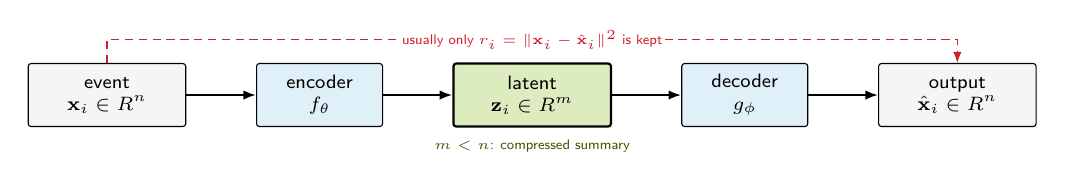
\begin{tikzpicture}[x=1mm,y=1mm,
      box/.style={draw, rounded corners=1pt, minimum height=8mm, align=center, font=\scriptsize},
      arr/.style={-{Latex[length=1.6mm]}, thick}]
    \node[box, fill=black!4,         minimum width=20mm] (x)   at (0,0)   {event\\$\mathbf{x}_i\in\mathbb{R}^{n}$};
    \node[box, fill=argonneBlue!12,  minimum width=16mm] (enc) at (27,0)  {encoder\\$f_\theta$};
    \node[box, fill=argonneGreen!25, minimum width=20mm, thick] (z) at (54,0) {latent\\$\mathbf{z}_i\in\mathbb{R}^{m}$};
    \node[box, fill=argonneBlue!12,  minimum width=16mm] (dec) at (81,0)  {decoder\\$g_\phi$};
    \node[box, fill=black!4,         minimum width=20mm] (xh)  at (108,0) {output\\$\hat{\mathbf{x}}_i\in\mathbb{R}^{n}$};
    \draw[arr] (x) -- (enc);
    \draw[arr] (enc) -- (z);
    \draw[arr] (z) -- (dec);
    \draw[arr] (dec) -- (xh);
    \node[font=\tiny, text=argonneGreen!50!black] at (54,-6.5) {$m<n$: compressed summary};
    \draw[argonneRed, densely dashed, -{Latex[length=1.4mm]}]
      (x.north) -- ++(0,3) -| (xh.north);
    \node[font=\tiny, text=argonneRed, fill=white, inner sep=1pt] at (54,7)
      {usually only $r_i=\|\mathbf{x}_i-\hat{\mathbf{x}}_i\|^2$ is kept};
  \end{tikzpicture}

  \vspace{5mm}
  \begin{columns}[T,onlytextwidth]
    \begin{column}{0.47\textwidth}
      {\small\textbf{What the autoencoder learns}}\par
      {\footnotesize
      \setlength{\abovedisplayskip}{3pt}\setlength{\belowdisplayskip}{0pt}
      \begin{gather*}
        \mathbf{z}_i = f_\theta(\mathbf{x}_i)\in\mathbb{R}^{m},\qquad
        \hat{\mathbf{x}}_i = g_\phi(\mathbf{z}_i)\in\mathbb{R}^{n}\\[1mm]
        \min_{\theta,\phi}\;\frac{1}{N}\sum_{i=1}^{N}\big\|\mathbf{x}_i-g_\phi(f_\theta(\mathbf{x}_i))\big\|_2^2
      \end{gather*}\par}
    \end{column}

    \begin{column}{0.49\textwidth}
      {\small\textbf{Why look at $\mathbf{z}_i$?}}\par
      \begin{itemize}
        \tightlist
        \item $r_i$: one number per event
        \item $\mathbf{z}_i$: a structured, $m$-dim description
        \item Similar $r_i$ can hide very different events
      \end{itemize}
    \end{column}
  \end{columns}

  \vspace{3.0mm}
  \takeaway{$\mathbf{z}_i$ carries more information than the 1D error $r_i$.}

  \slideheaderfooter
\end{frame}

% ============================================================
%  Slide 2: t-SNE view of learned jet embeddings
% ============================================================
\begin{frame}[plain]
  \slideheader{Visualizing jet embeddings}
  \setbeamerfont{itemize/enumerate body}{size=\footnotesize}

  \vfill
  \begin{columns}[c,onlytextwidth]
    \begin{column}{0.66\textwidth}
      \centering
      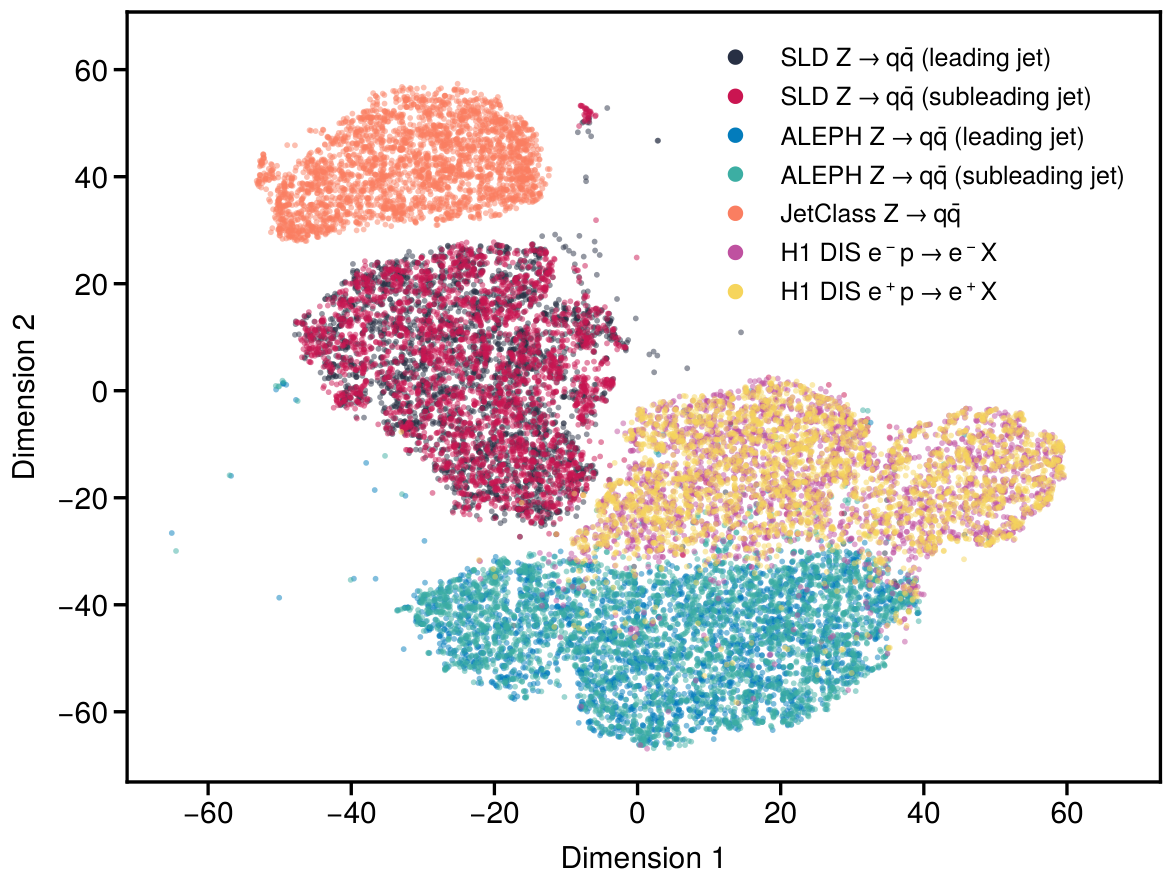
\includegraphics[width=\linewidth,height=48mm,keepaspectratio]{figures/embedding_tsne_m.png}

      {\tiny\textit{Fig.~6, arXiv:2606.00224: t-SNE visualization of OmniLearned jet embeddings.}\par}
    \end{column}

    \begin{column}{0.30\textwidth}
      {\small\textbf{t-SNE of jet embeddings}}\par
      \begin{itemize}
        \setlength{\itemsep}{0.8mm}
        \item Learned jet embeddings are projected to 2D for visualization.
        \item Jets with similar learned features appear nearby.
        \item Similar physics topologies group together in embedding space.
      \end{itemize}
    \end{column}
  \end{columns}
  \vfill

  \slideheaderfooter
\end{frame}

% ============================================================
%  Slide 3: Grouping anomalous events in latent space
% ============================================================
\begin{frame}[plain]
  \slideheader{Are anomalies alike?}
  \setbeamerfont{itemize/enumerate body}{size=\footnotesize}

  \vspace{12mm}
  \begin{columns}[c,onlytextwidth]
    \begin{column}{0.46\textwidth}
      \begin{enumerate}
        \tightlist
        \item Flag events with large error: $r_i>\tau$.
        \item Take their latent vectors $\mathbf{z}_i$.
        \item Project with t-SNE and highlight the flagged events.
      \end{enumerate}

      \vspace{1.5mm}
      \begin{itemize}
        \tightlist
        \item \textcolor{argonneRed}{\textbf{Packed together}}: anomalies look alike
              $\Rightarrow$ likely a common source.
        \item \textcolor{argonneGreen!70!black}{\textbf{Isolated}}: a one-off
              unusual event.
        \item Different clusters $\Rightarrow$ different kinds of anomaly.
      \end{itemize}
    \end{column}

    \begin{column}{0.50\textwidth}
      \centering
      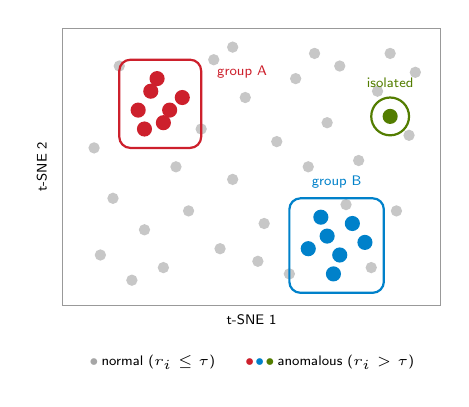
\begin{tikzpicture}[x=0.8mm,y=0.8mm]
        \draw[black!40] (0,0) rectangle (60,44);
        \node[font=\tiny, below] at (30,0) {t-SNE 1};
        \node[font=\tiny, rotate=90, anchor=south] at (-1,22) {t-SNE 2};

        % normal events (low r_i)
        \foreach \x/\y in {6/8,8/17,13/12,20/15,22/28,25/9,27/20,29/33,32/13,34/26,37/36,
                           39/22,42/29,47/23,50/34,53/15,55/27,16/6,24/39,31/7,40/40,49/6,
                           56/37,5/25,36/5,44/38,9/38,27/41,18/22,45/16,52/40,11/4}
          {\fill[black!22] (\x,\y) circle (0.9);}

        % anomaly cluster A
        \foreach \x/\y in {12/31,14/34,17/31,15/36,19/33,13/28,16/29}
          {\fill[argonneRed] (\x,\y) circle (1.2);}
        \draw[argonneRed, thick, rounded corners] (9,25) rectangle (22,39);
        \node[font=\tiny, text=argonneRed, anchor=west] at (23,37) {group A};

        % anomaly cluster B
        \foreach \x/\y in {39/9,42/11,44/8,46/13,41/14,48/10,43/5}
          {\fill[argonneBlue] (\x,\y) circle (1.2);}
        \draw[argonneBlue, thick, rounded corners] (36,2) rectangle (51,17);
        \node[font=\tiny, text=argonneBlue, anchor=south] at (43.5,17) {group B};

        % isolated anomaly
        \fill[argonneGreen!70!black] (52,30) circle (1.2);
        \draw[argonneGreen!70!black, thick] (52,30) circle (3);
        \node[font=\tiny, text=argonneGreen!70!black, anchor=south] at (52,33) {isolated};

        % legend
        \node[font=\tiny] at (30,-9)
          {\textcolor{black!35}{$\bullet$}\,normal ($r_i\le\tau$)\qquad
           \textcolor{argonneRed}{$\bullet$}\textcolor{argonneBlue}{$\bullet$}\textcolor{argonneGreen!70!black}{$\bullet$}\,anomalous ($r_i>\tau$)};
      \end{tikzpicture}

    \end{column}
  \end{columns}

  \vspace{6.0mm}
  {\centering\color{black}\itshape Conclusion: $r_i$ flags anomalies; latent space shows which belong together.\par}

  \slideheaderfooter
\end{frame}


% Optional backup section pattern:
% \setmainframenumber
% \appendix
% \input{src/backup.tex}

\end{document}
